\chapter{Uso de Tecnologias Digitais} % (fold)
\label{chap:Conteúdo Programático}
O planejamento do professor supervisor não foi disponibilizado, o mesmo é postado no sistema da escola no início de cada ano, no entanto, foi possível acompanhar atualizações contínuas em ambiente virtual \textit{Google Classroom} para cada uma de suas turmas, assim promove o uso das \ac{TICs}. Neste ambiente o professor posta atividades, vídeos adcionais e materiais complementares para as suas aulas. A seguir apresentaremos o material disponibilizado até o mês de julho para as turmas de 1ª e 2ª Séries do \ac{NEM} e 3ª Série do \ac{EM}.

\section{Primeira Série} % (fold)
Na turma de 1º Série -- 5 do \ac{NEM} os tópicos disponibilizados no G. Classroom para este primeiro semestre foram os seguintes:
\vspace{10pt}

\begin{figure}[!ht]
	\centering
	\caption{Ambiente Virtual -- 1(5) noturno}
	\label{fig:prog-1_cinco}
	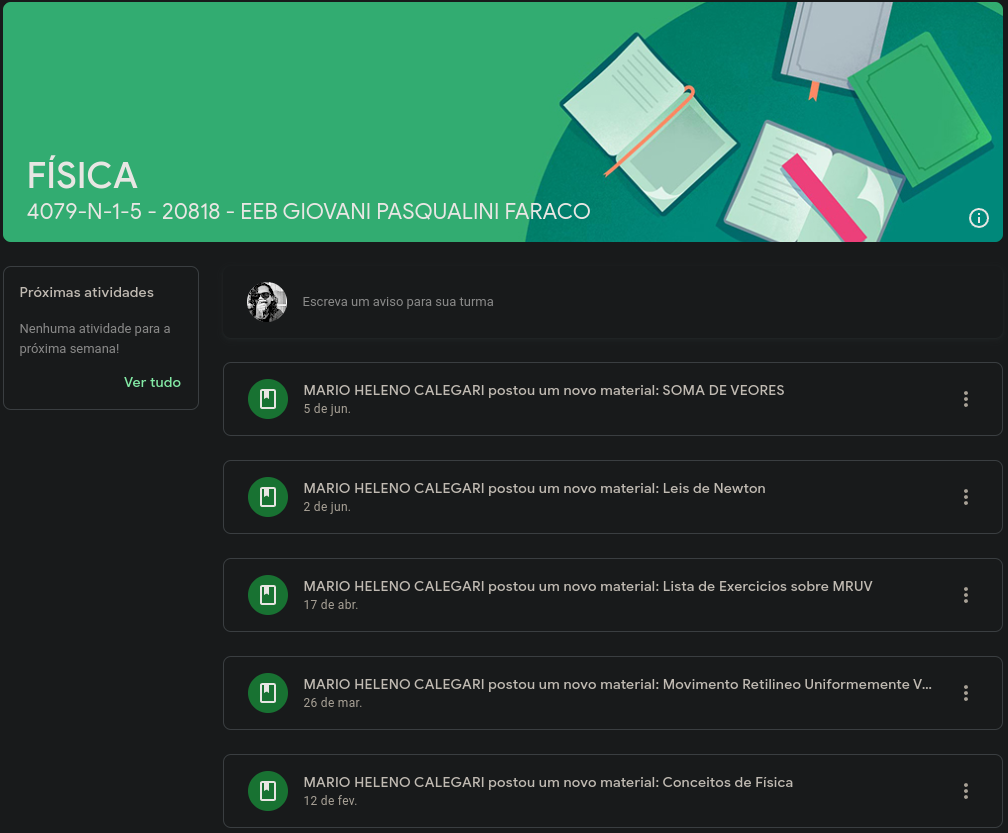
\includegraphics[width=.8\textwidth]{assets/conteudo_programatico-1.png}
	\legend{Fonte: G. Classrom da turma}
\end{figure}

\begin{enumerate}
	\item Conceitos de Física;
	\item Movimento Retilíneo Uniformemente Variável;
	\item Exercício sobre MRUV;
	\item Leis de Newton;
	\item Soma de Vetores.
\end{enumerate}
Um \textit{printscreen} do ambiente virtual da turma pode ser visto na \autoref{fig:prog-1_cinco} a seguir:


Identifica-se na sequência o ordenamento de assuntos partindo do simples ao complexo. Nesta estrutura o professor aborda os temas sequencialmente e a medida que avança pelos tópicos vai acescentando novos elementos. Esta estrutura é padrão nos livros especializados da disciplina. 
% section Primeira Série (end)

\section{Segunda Série} % (fold)
\label{sec:Segunda Série}
Para a turma da 2ª Série -- 6 do \ac{NEM} verificou-se um padrão semelhante ao da turma anterior. Um \textit{printscreen} do ambiente virtual desta turma é visto na \autoref{fig:prog-2_seis}.
\vspace{10pt}
\begin{figure}[!ht]
	\centering
	\caption{Ambiente Virtual -- 2(6) noturno}
	\label{fig:prog-2_seis}
	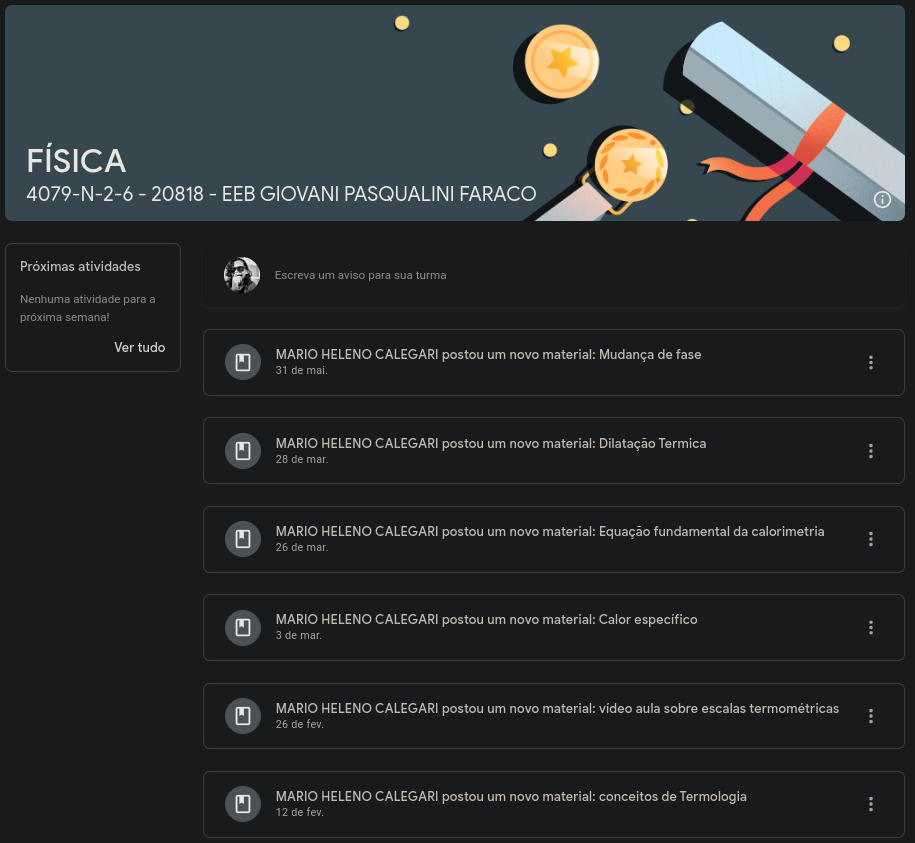
\includegraphics[width=.8\linewidth]{assets/conteudo_programatico-2.png}
	\legend{Fonte: G. Classrom da turma}
\end{figure}

\noindent Nesta turma, os conteúdos abordados foram na sequência:
\begin{enumerate}
	\item Termologia;
	\item Escalas Termométricas;
	\item Calor Específico;
	\item Equação Fundamental da Calorimetria;
	\item Dilatação Térmica;
	\item Mudança de Fase.
\end{enumerate}
% section Segunda Série (end)

\section{Terceira Série} % (fold)
\label{sec:Terceiro Série}
Com a turma da 3ª Série -- 4 do \ac{EM} não foi diferente, um \textit{printscreen} do G. Classroom desta turma é visto na \autoref{fig:prog-3_quatro} a seguir:
\vspace{10pt}
\begin{figure}[!ht]
	\centering
	\caption{Ambiente Virtual -- 3(4) noturno}
	\label{fig:prog-3_quatro}
	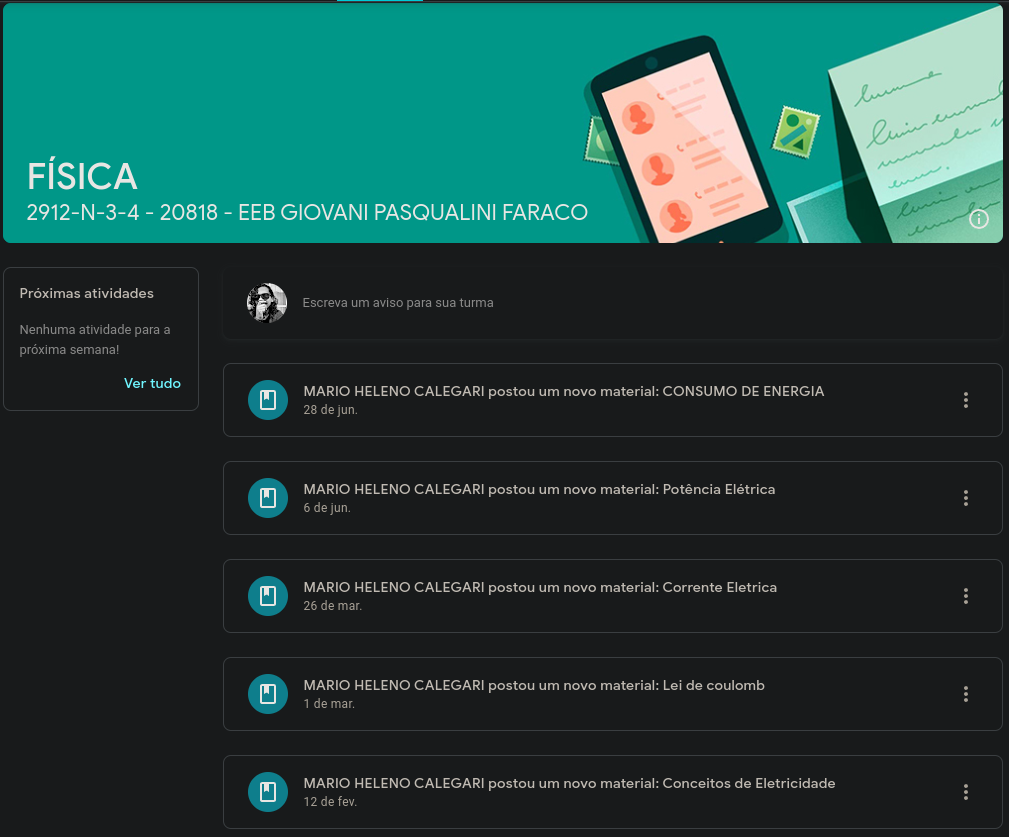
\includegraphics[width=.8\linewidth]{assets/conteudo_programatico-3.png}
	\legend{Fonte: G. Clasroom da turma}
\end{figure}

\noindent Para esta turma, os conteúdos abordados foram na sequência:
\begin{enumerate}
	\item Conceitos de Eletricidade;
	\item Lei de Coulomb;
	\item Corrente Elétrica;
	\item Potência Elétrica;
	\item Consumo de Energia.
\end{enumerate}

% section Terceira Série (end)

% chapter Conteúdo Programático (end)
